\section{Answers to questions}

\subsection{Question 1}
\textit{Run the three algorithms you have implemented (2-Approximation, Nearest Neighbor and Closest Insertion) on the 13 graphs of the dataset. Show your results in a table. The rows in the table correspond to the problem instances. The columns show, for each algorithm, the weight of the approximate solution, the execution time and the relative error calculated as:
\[\frac{(ApproximateSolution - OptimalSolution)}{OptimalSolution}\]}\\

\noindent
We have implemented the code in C\# for the execution of the three algorithms on the whole provided dataset.
In the following table we show the optimal solutions for the datasets as reference for the results that we obtain.
\begin{table}[H]\centering
    \begin{tabular}{|l|l|r|r|}
    \hline
    \textbf{File} & \textbf{Description} & \textbf{N} & \textbf{Optimal solution} \\
    \hline
    \textit{burma14.tsp}	    & Burma (Myanmar)	& 14	& 3323 \\
    \textit{ulysses16.tsp}      & Mediterranean Sea & 16	& 6859 \\
    \textit{ulysses22.tsp}      & Mediterranean Sea & 22	& 7013 \\
    \textit{eil51.tsp}          & Synthetic	        & 51	& 426 \\
    \textit{berlin52.tsp}	    & Germany	        & 52 	& 7542 \\
    \textit{kroD100.tsp}	    & Random	        & 100	& 21294 \\
    \textit{kroA100.tsp}	    & Random 	        & 100	& 21282 \\
    \textit{ch150.tsp}	        & Random	        & 150	& 6528 \\
    \textit{gr202.tsp}	        & Europe	        & 202   & 40160 \\
    \textit{gr229.tsp}	        & Asia/Australia	& 229	& 134602 \\
    \textit{pcb442.tsp}         & Drilling		    & 442 	& 50778 \\
    \textit{d493.tsp}	        & Drilling	        & 493	& 35002 \\
    \textit{dsj1000.tsp}	    & Random	        & 1000 	& 18659688 \\
    \hline
    \end{tabular}
    \caption{Optimal solution for each dataset.}
\end{table}

\subsubsection{Results}
The results of our implemented algorithms are show in the table at the following page.
\begin{landscape}
\begin{table}\centering
    \begin{tabular}{|l|r|r|c|r|r|c|r|r|c|}
    \hline
    \multicolumn{1}{|c|}{\multirow{2}{*}{\textbf{Instance}}} & \multicolumn{3}{c|}{\textbf{Nearest Neighbour}} & \multicolumn{3}{c|}{\textbf{Closest Insertion}} & \multicolumn{3}{c|}{\textbf{2-Approximation}} \\ \cline{2-10} 
    \multicolumn{1}{|c|}{} & \multicolumn{1}{c|}{\textbf{Solution}} & \multicolumn{1}{c|}{\textbf{\begin{tabular}[c]{@{}c@{}}Time\\ {[}ms{]}\end{tabular}}} & \multicolumn{1}{c|}{\textbf{\begin{tabular}[c]{@{}c@{}}Error\\ {[}\%{]}\end{tabular}}} & \multicolumn{1}{c|}{\textbf{Solution}} & \multicolumn{1}{c|}{\textbf{\begin{tabular}[c]{@{}c@{}}Time \\ {[}ms{]}\end{tabular}}} & \multicolumn{1}{c|}{\textbf{\begin{tabular}[c]{@{}c@{}}Error\\ {[}\%{]}\end{tabular}}} & \multicolumn{1}{c|}{\textbf{Solution}} & \multicolumn{1}{c|}{\textbf{\begin{tabular}[c]{@{}c@{}}Time\\ {[}ms{]}\end{tabular}}} & \multicolumn{1}{c|}{\textbf{\begin{tabular}[c]{@{}c@{}}Error\\ {[}\%{]}\end{tabular}}} \\ \hline
  
    \hline
    
    \textit{burma14.tsp}	& 4048	    & 0,03	    & 21,82 	& 3588	    & 0,148	    & 7,97      & 3814	    & 0,037	    & 14,78 \\
    \textit{ulysses16.tsp}	& 9988	    & 0,04	    & 45,62 	& 7712	    & 0,212	    & 12,44 	& 7903	    & 0,049	    & 15,22 \\
    \textit{ulysses22.tsp}	& 10586	    & 0,076	    & 50,95     & 7816	    & 0,491	    & 11,45     & 8401	    & 0,088	    & 19,79 \\
    \textit{eil51.tsp}	    & 511	    & 0,408	    & 19,95 	& 494	    & 4,934	    & 15,96 	& 581	    & 0,452	    & 36,38 \\
    \textit{berlin52.tsp}	& 8980	    & 0,426	    & 19,07 	& 8991	    & 5,104	    & 19,21 	& 10114	    & 0,492	    & 34,10 \\
    \textit{kroD100.tsp}    & 26947	    & 1,589	    & 26,55 	& 25219	    & 34,317	& 18,43 	& 27112	    & 1,835	    & 27,32 \\    
    \textit{kroA100.tsp}	& 27807	    & 1,601	    & 30,66 	& 25868	    & 33,802	& 21,55 	& 27210	    & 1,8       & 27,85 \\
    \textit{ch150.tsp}	    & 8191	    & 3,647	    & 25,47 	& 7968	    & 115,24	& 22,06 	& 8413	    & 4,194 	& 28,88 \\
    \textit{gr202.tsp}	    & 49336	    & 6,65  	& 22,85 	& 47170	    & 280,744	& 17,46 	& 51990	    & 7,547 	& 29,46 \\
    \textit{gr229.tsp}	    & 162430	& 8,726 	& 20,67 	& 156823	& 421,81	& 16,51     & 180152	& 9,822 	& 33,84 \\
    \textit{pcb442.tsp}	    & 61979	    & 39,297	& 22,06 	& 61119	    & 3.089,46	& 20,37 	& 69623	    & 43,674	& 37,11 \\
    \textit{d493.tsp}	    & 41660	    & 43,028	& 19,02 	& 41459	    & 4.010,31	& 18,45 	& 44953	    & 48,732	& 28,43 \\
    \textit{dsj1000.tsp}	& 24630960	& 266,321	& 32,00 	& 22723503	& 42.221,13	& 21,78 	& 25086767	& 322,979	& 34,44 \\

    \hline
    \end{tabular}
    \caption{Results of execution of the three algorithm on datasets.}
\end{table}
\end{landscape}
\noindent
We believe it is useful to report in detail the execution times of the algorithms and the number of repetitions performed in one second by each algorithm on each dataset.
\begin{table}[H]\centering
    \begin{tabular}{|l|l|r|r|r|r|r|r|}
    \hline
    \textbf{File} & \textbf{N} & \textbf{\begin{tabular}[c]{@{}c@{}}Time NN\\ {[}ms{]}\end{tabular}} & \textbf{Rep NN} & \textbf{\begin{tabular}[c]{@{}c@{}}Time CI\\ {[}ms{]}\end{tabular}} & \textbf{Rep CI} & \textbf{\begin{tabular}[c]{@{}c@{}}Time 2-AP\\ {[}ms{]}\end{tabular}} & \textbf{Rep 2-AP} \\
    \hline

    \textit{burma14.tsp}	    & 14	& 0,03  	& 32865     & 0,148	    & 6760  & 0,037	    & 26912 \\
    \textit{ulysses16.tsp}      & 16	& 0,04	    & 25148     & 0,212	    & 4716  & 0,049	    & 20425 \\
    \textit{ulysses22.tsp}      & 22	& 0,076	    & 13163     & 0,491	    & 2036  & 0,088	    & 11302 \\
    \textit{eil51.tsp}          & 51	& 0,408	    & 2450      & 4,934	    & 203   & 0,452	    & 2212 \\
    \textit{berlin52.tsp}	    & 52 	& 0,426 	& 2348      & 5,104	    & 196   & 0,492	    & 2033 \\
    \textit{kroD100.tsp}	    & 100	& 1,589	    & 630       & 34,317	& 30    & 1,835	    & 545 \\
    \textit{kroA100.tsp}	    & 100	& 1,601	    & 625       & 33,802	& 30    & 1,8	    & 556 \\
    \textit{ch150.tsp}	        & 150	& 3,647 	& 275       & 115,24	& 9     & 4,194	    & 239 \\
    \textit{gr202.tsp}	        & 202   & 6,65	    & 151       & 280,744	& 4     & 7,547	    & 133 \\
    \textit{gr229.tsp}	        & 229	& 8,726	    & 115       & 421,81	& 3     & 9,822	    & 102 \\
    \textit{pcb442.tsp}         & 442 	& 39,297	& 26        & 3.089,46	& 1     & 43,674	& 23 \\
    \textit{d493.tsp}	        & 493	& 43,028	& 24        & 4.010,31	& 1     & 48,732	& 21 \\
    \textit{dsj1000.tsp}	    & 1000 	& 266,321	& 4         & 42.221,13	& 1     & 322,979	& 4 \\

    \hline
    \end{tabular}
    \caption{Approximated solution for each dataset.}
\end{table}

\subsection{Question 2}
\textit{Comment on the results you have obtained: how do the algorithms behave with respect to the various 
instances? There is an algorithm that is always better than the others? Which of the three algorithms you 
have implemented is more efficient?} \\

\noindent
Analyzing the three algorithm we saw that the more accurate is the \textit{Closest Insertion} algorithm, but as side effect is also the one that is the slowest.
As for the other two algorithms (Nearest neighbor and 2-Approximation) it is not clear which is the more precise: from the results we saw that 2-Approximation tends to be more precise in graph with small dimensions while nearest neighbor is able to find a better solution in graph with big dimension.\\
Below are some graphs showing the actual errors of the results and the errors in proportion to each other, in order to show what was discussed above.

\begin{figure}[H]
    \centering
    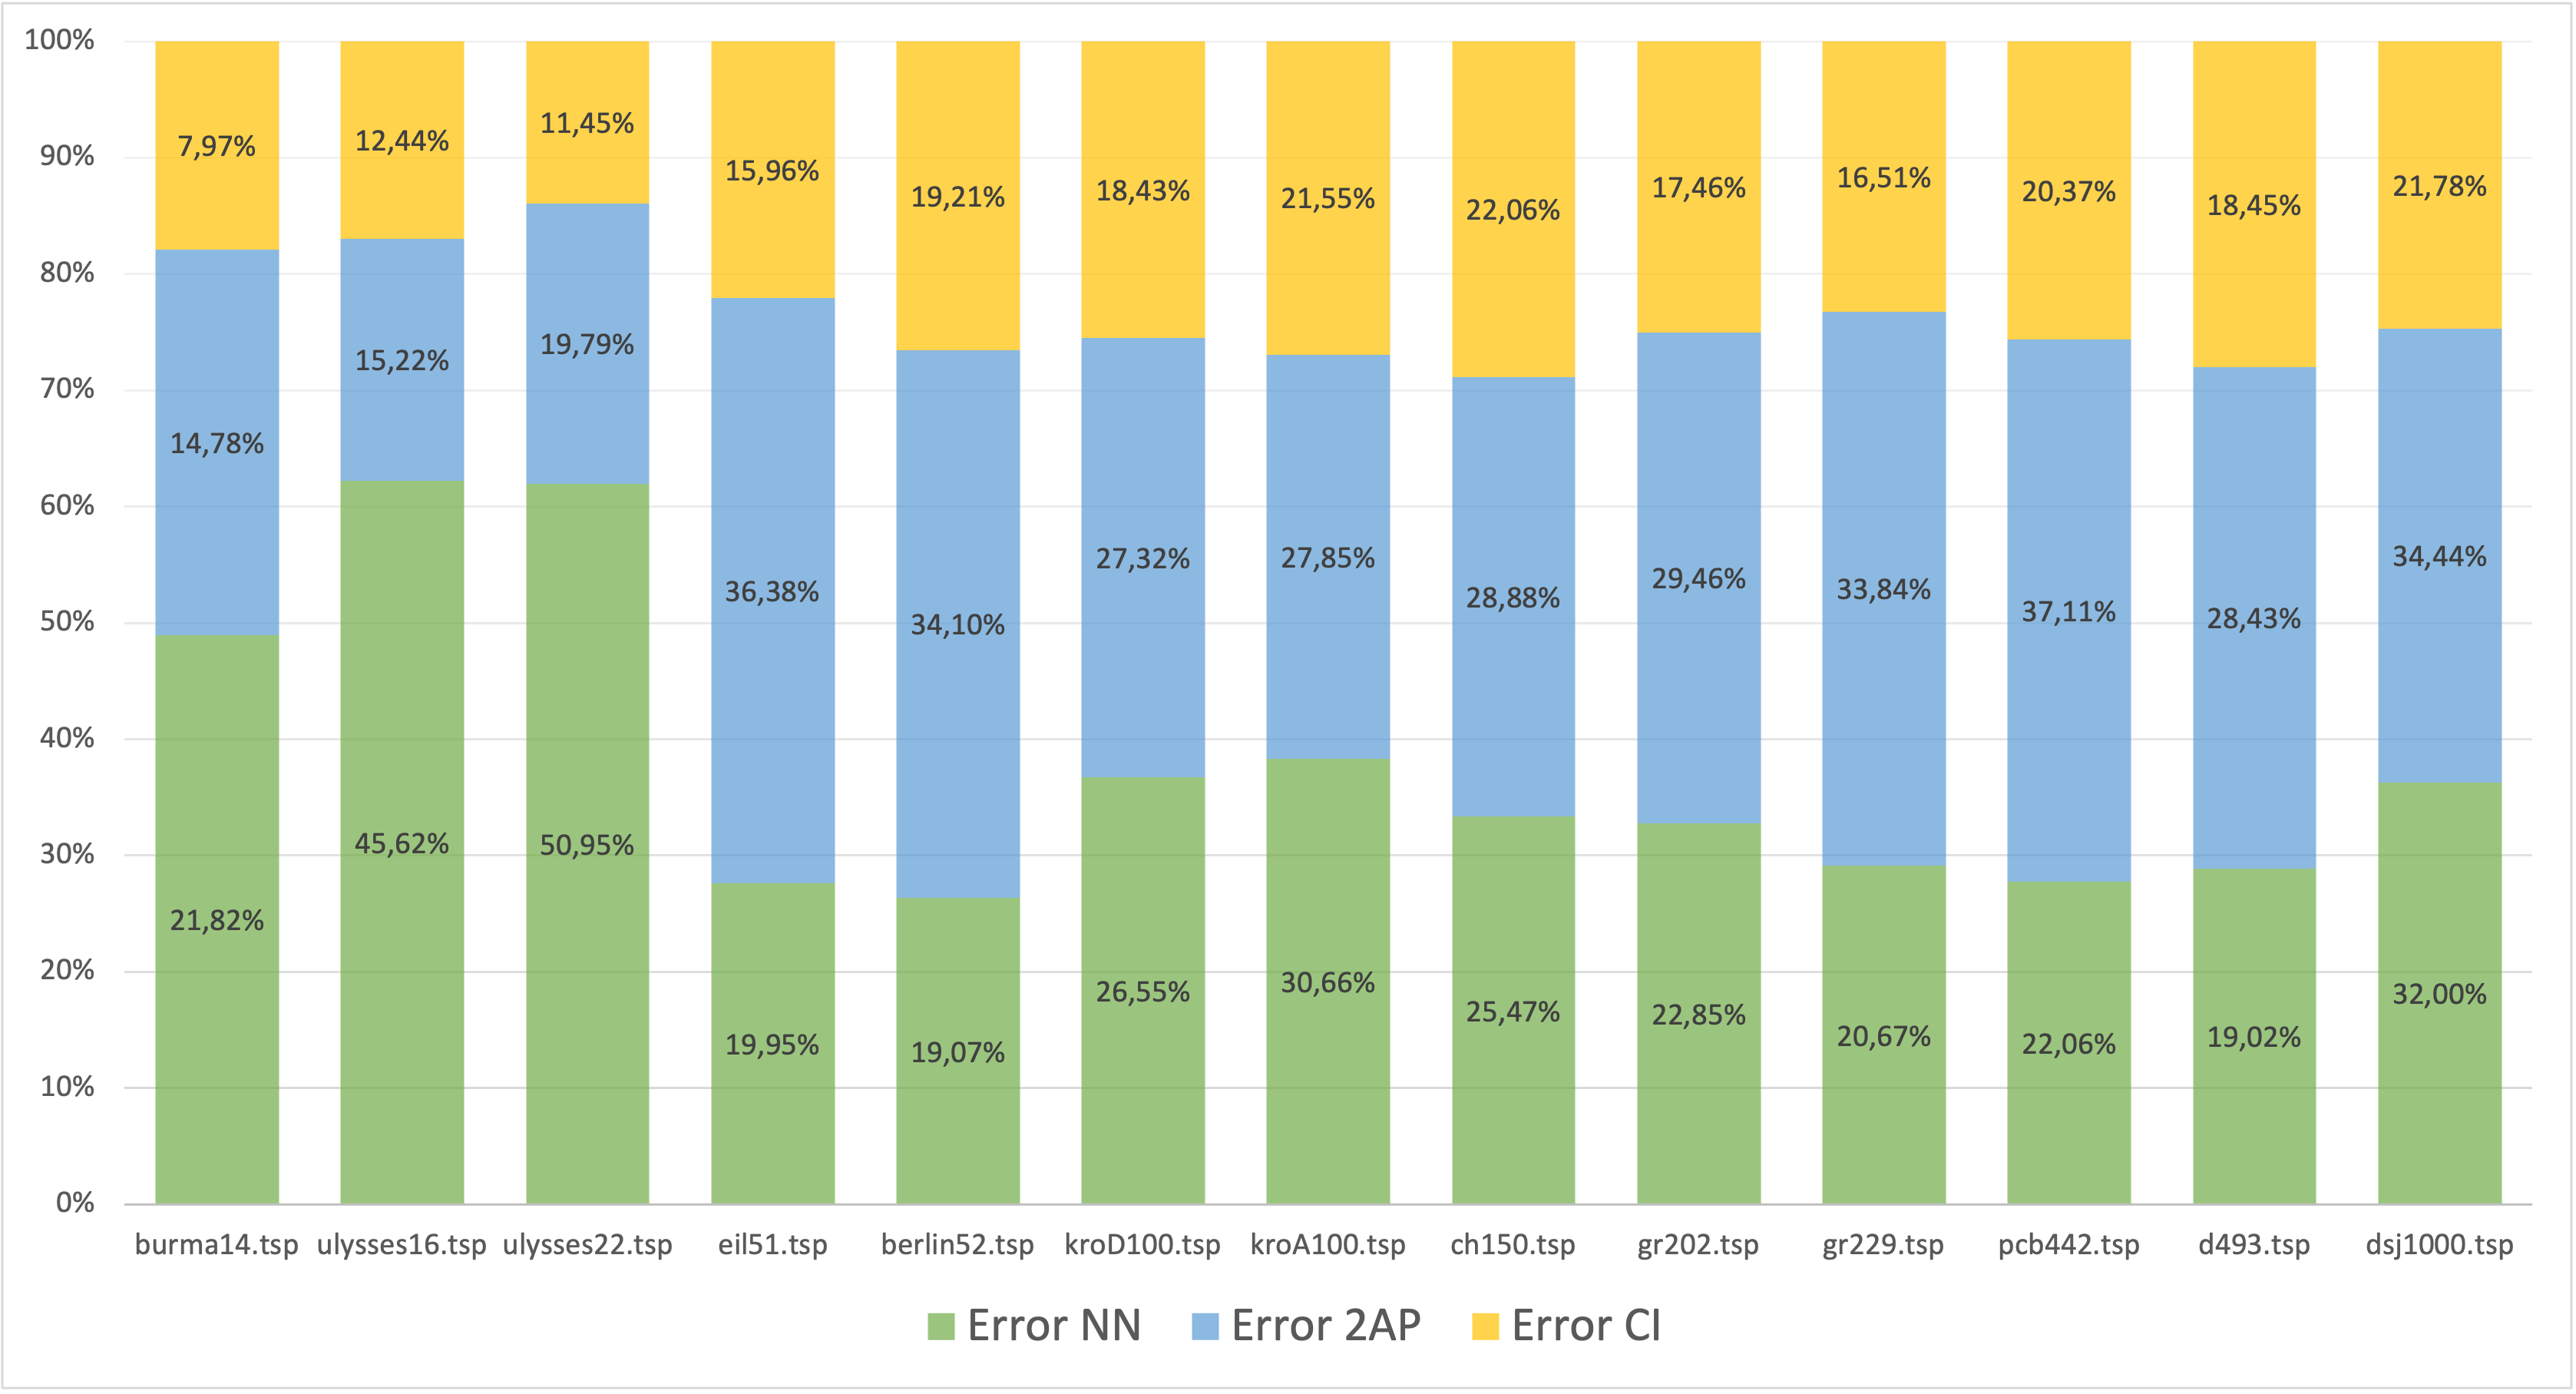
\includegraphics[width=0.9\textwidth]{./img/errore_in_proporzione_ord.png}
    \caption{Errors in proportion for the three algorithms.}
    \label{fig:proportion_error_ord}
\end{figure}

\begin{figure}[H]
    \centering
    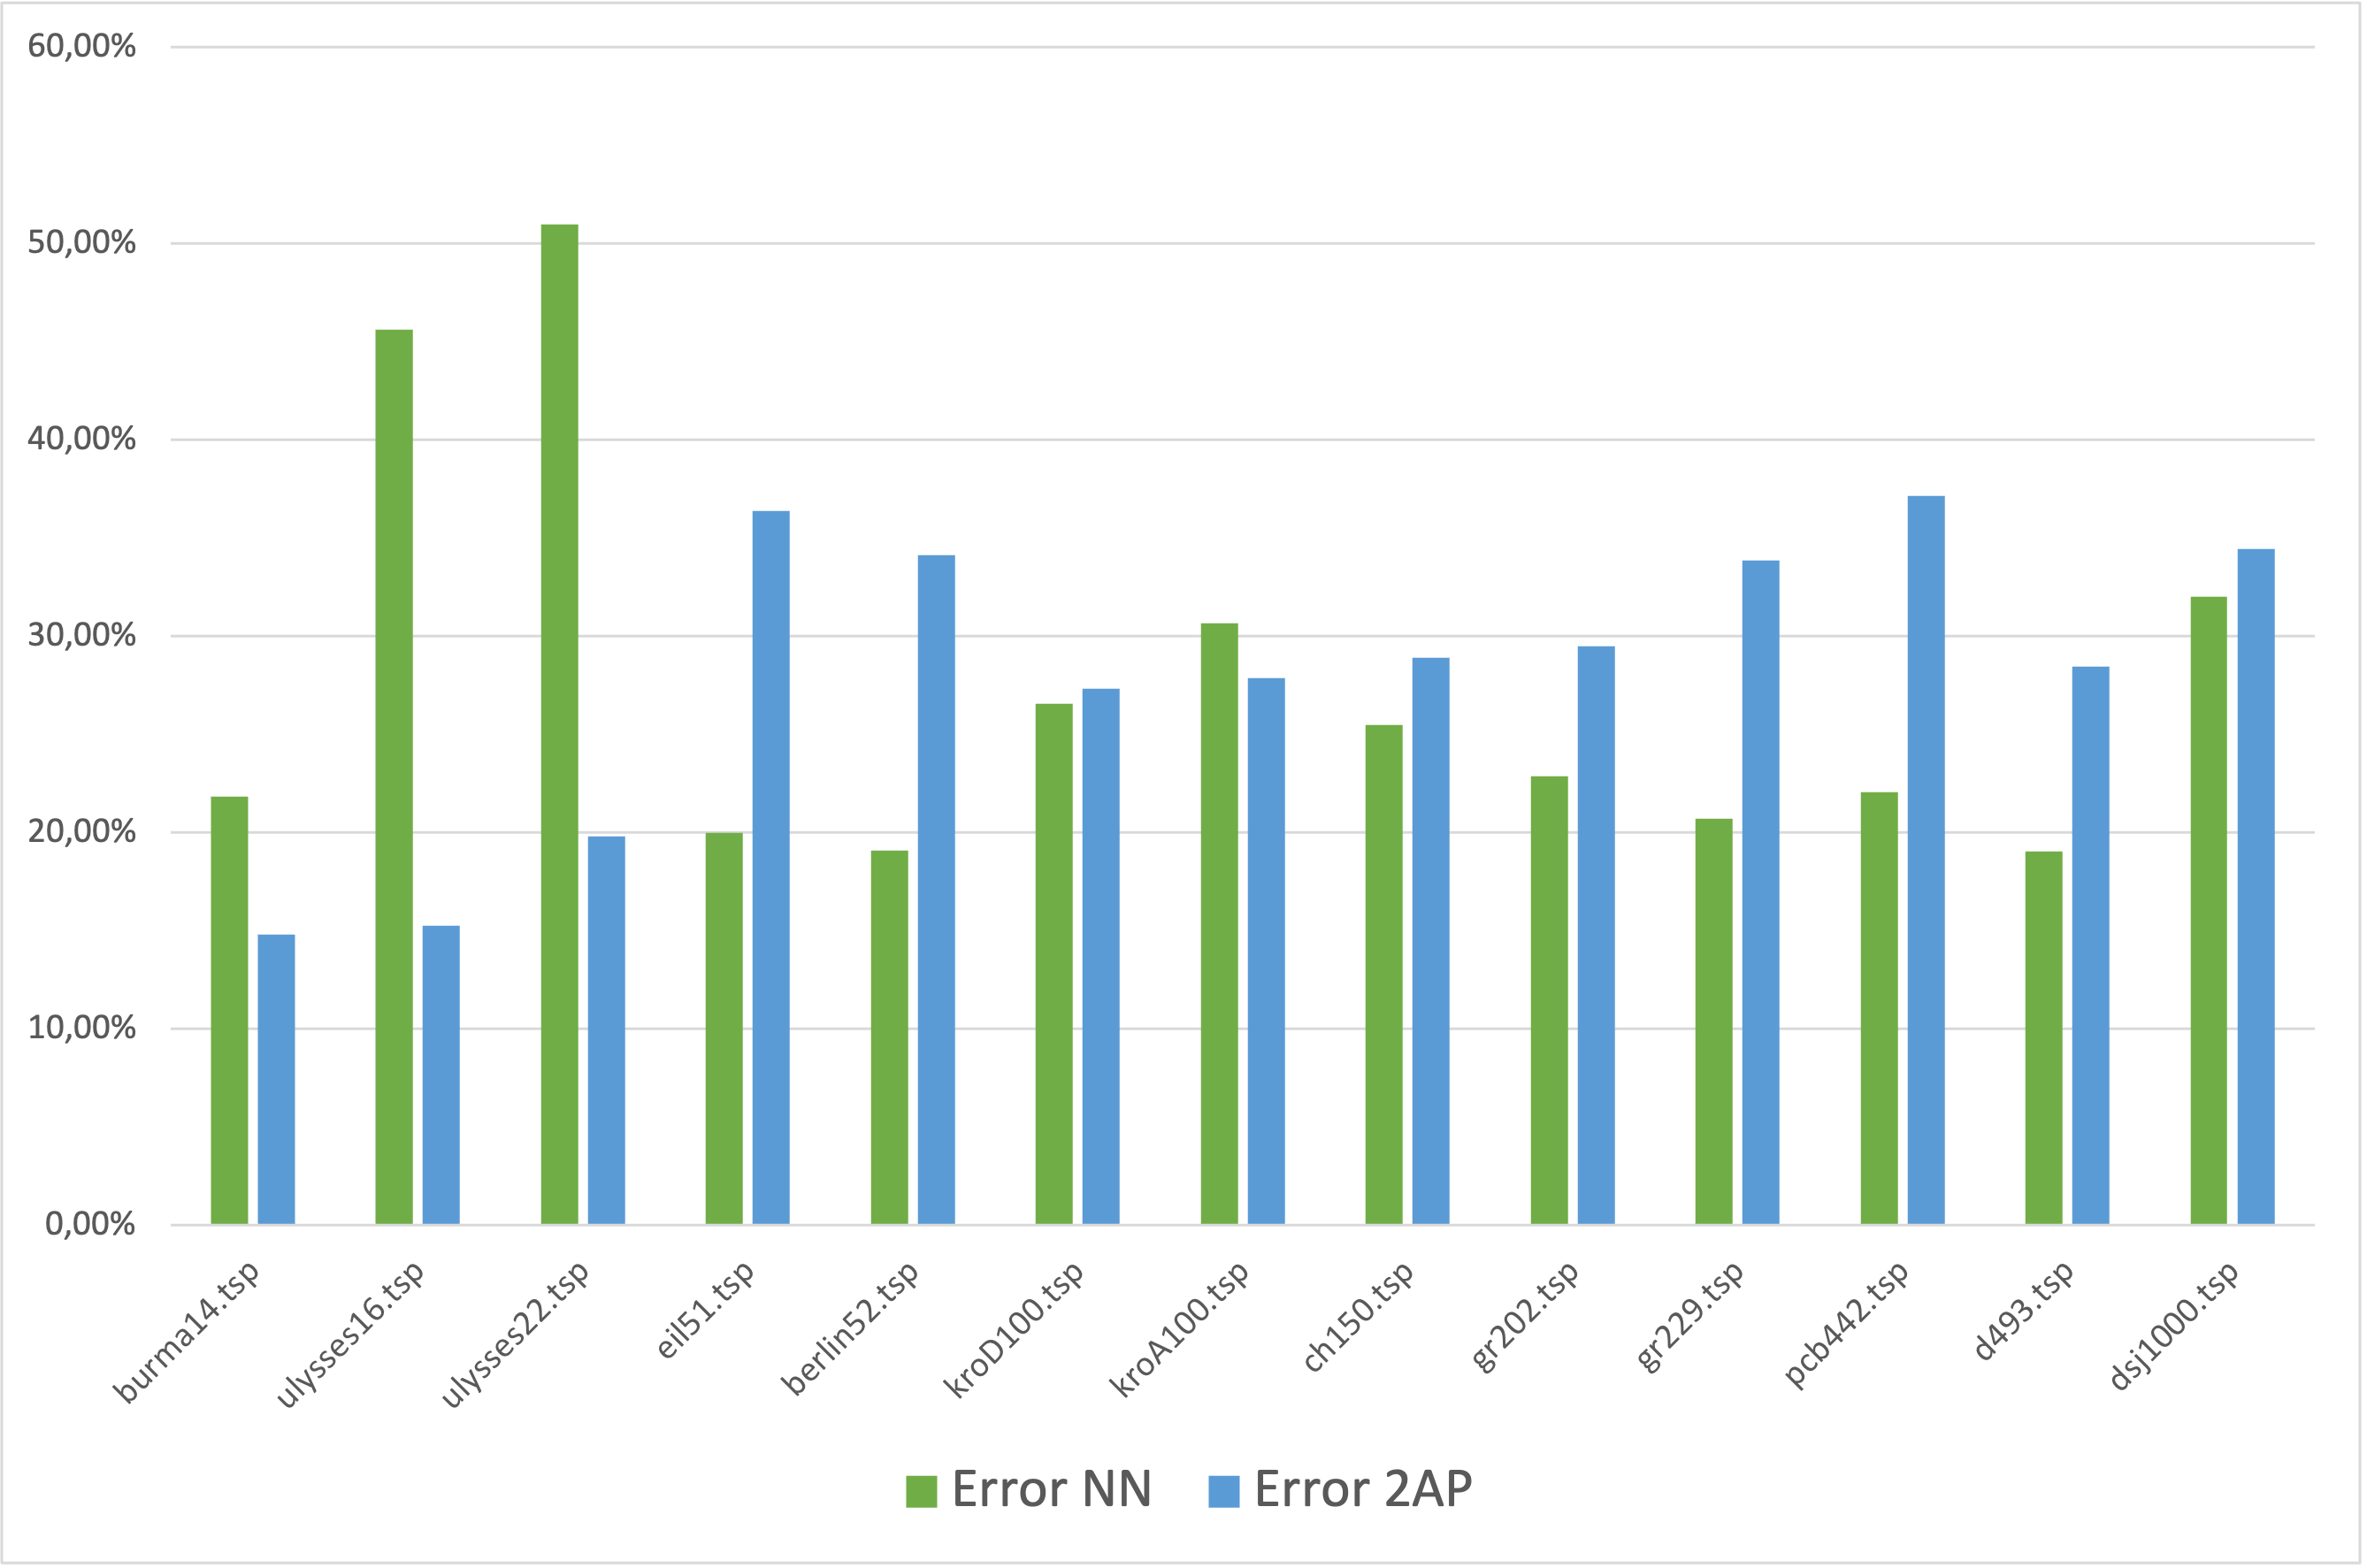
\includegraphics[width=0.9\textwidth]{./img/error_nn_2ap.png}
    \caption{Errors for Nearest Neighbor and 2-Approximation.}
    \label{fig:error_nn_2ap}
\end{figure}

\begin{figure}[H]
    \centering
    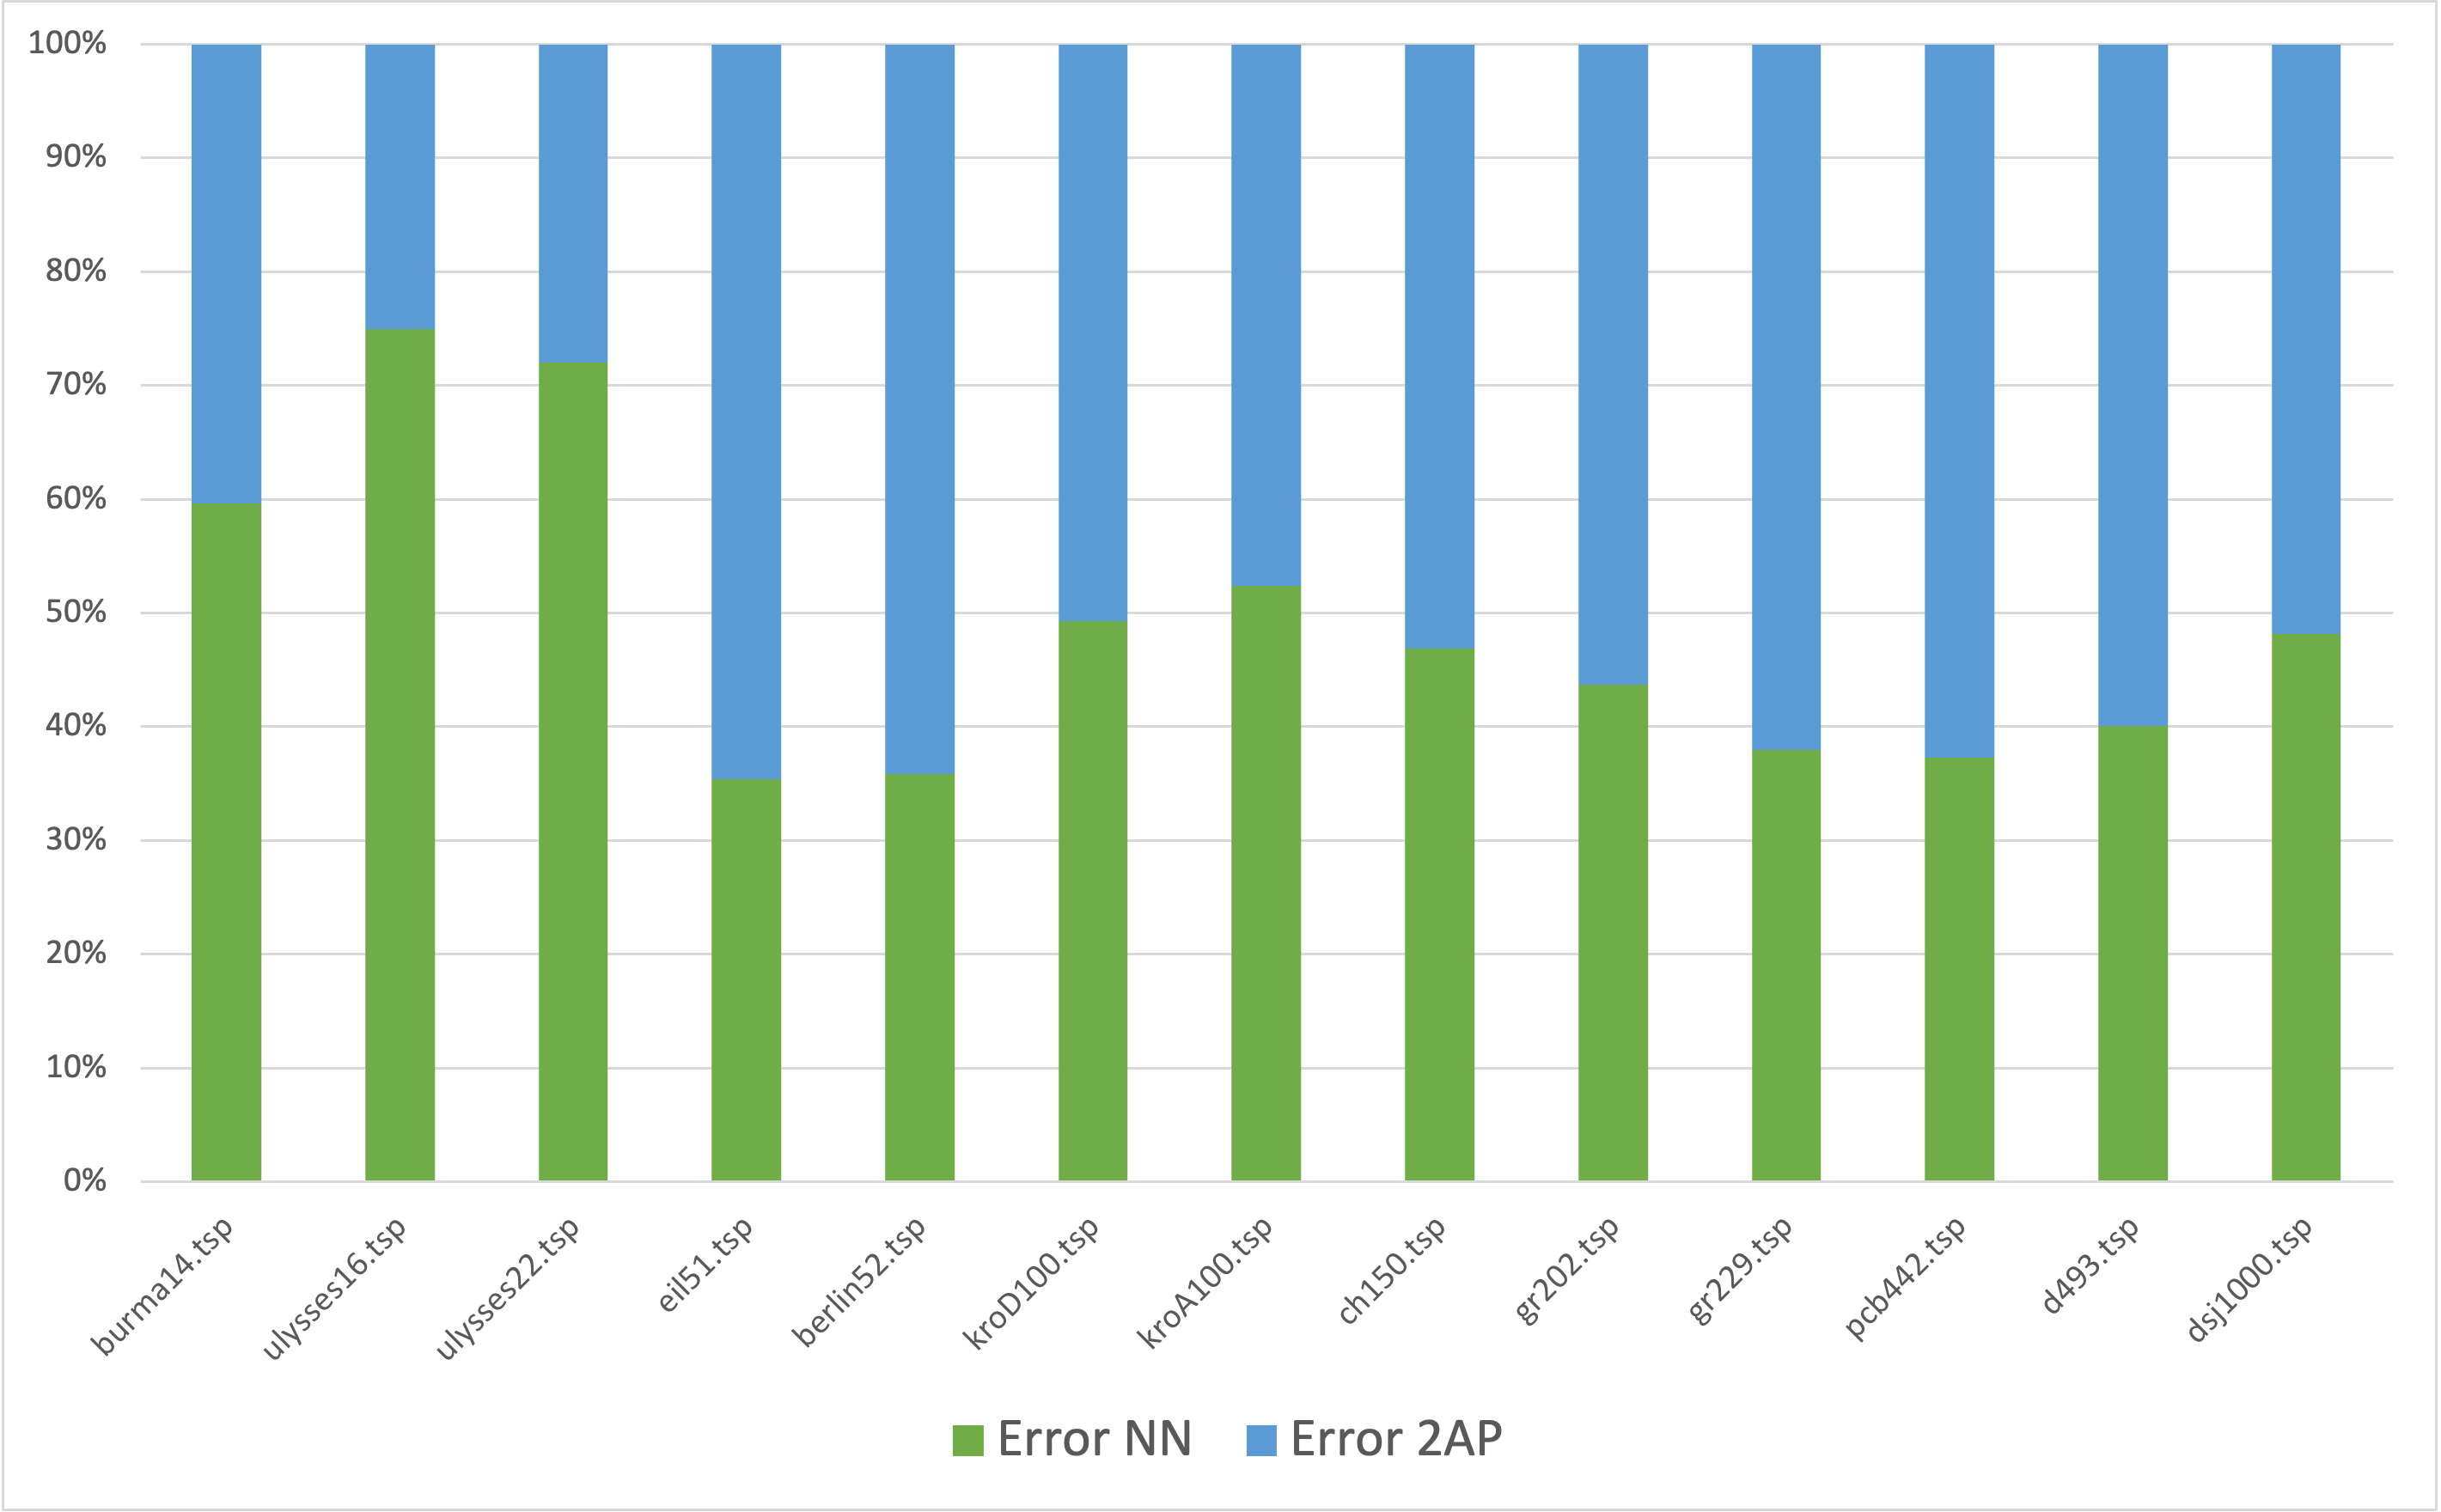
\includegraphics[width=0.9\textwidth]{./img/error_nn_2ap_prop.png}
    \caption{Errors in proportion for Nearest Neighbor and 2-Approximation.}
    \label{fig:error_nn_2ap_prop}
\end{figure}
\noindent
From the charts (fig. \ref{fig:proportion_error_ord}, \ref{fig:error_nn_2ap}, \ref{fig:error_nn_2ap_prop}) we can see that the \textit{Nearest Neighbor} algorithm seems to be, in mean, the most efficient. This is not true, in fact in the graph with small dimension, like (\textit{burma14}, \textit{ulysses16} and \textit{ulysses22}), the \textit{2-Approximation} algorithm is closest to the optimal solution than the Nearest Neighbor.\\
One thing we noticed is the fact that the Nearest Neighbor is a greedy algorithm and this may explain the fact that it performs well when the graph has big dimension and the number of choices that it has to compute is bigger and so the error rate decreases in proportion.

\begin{figure}[H]
    \centering
    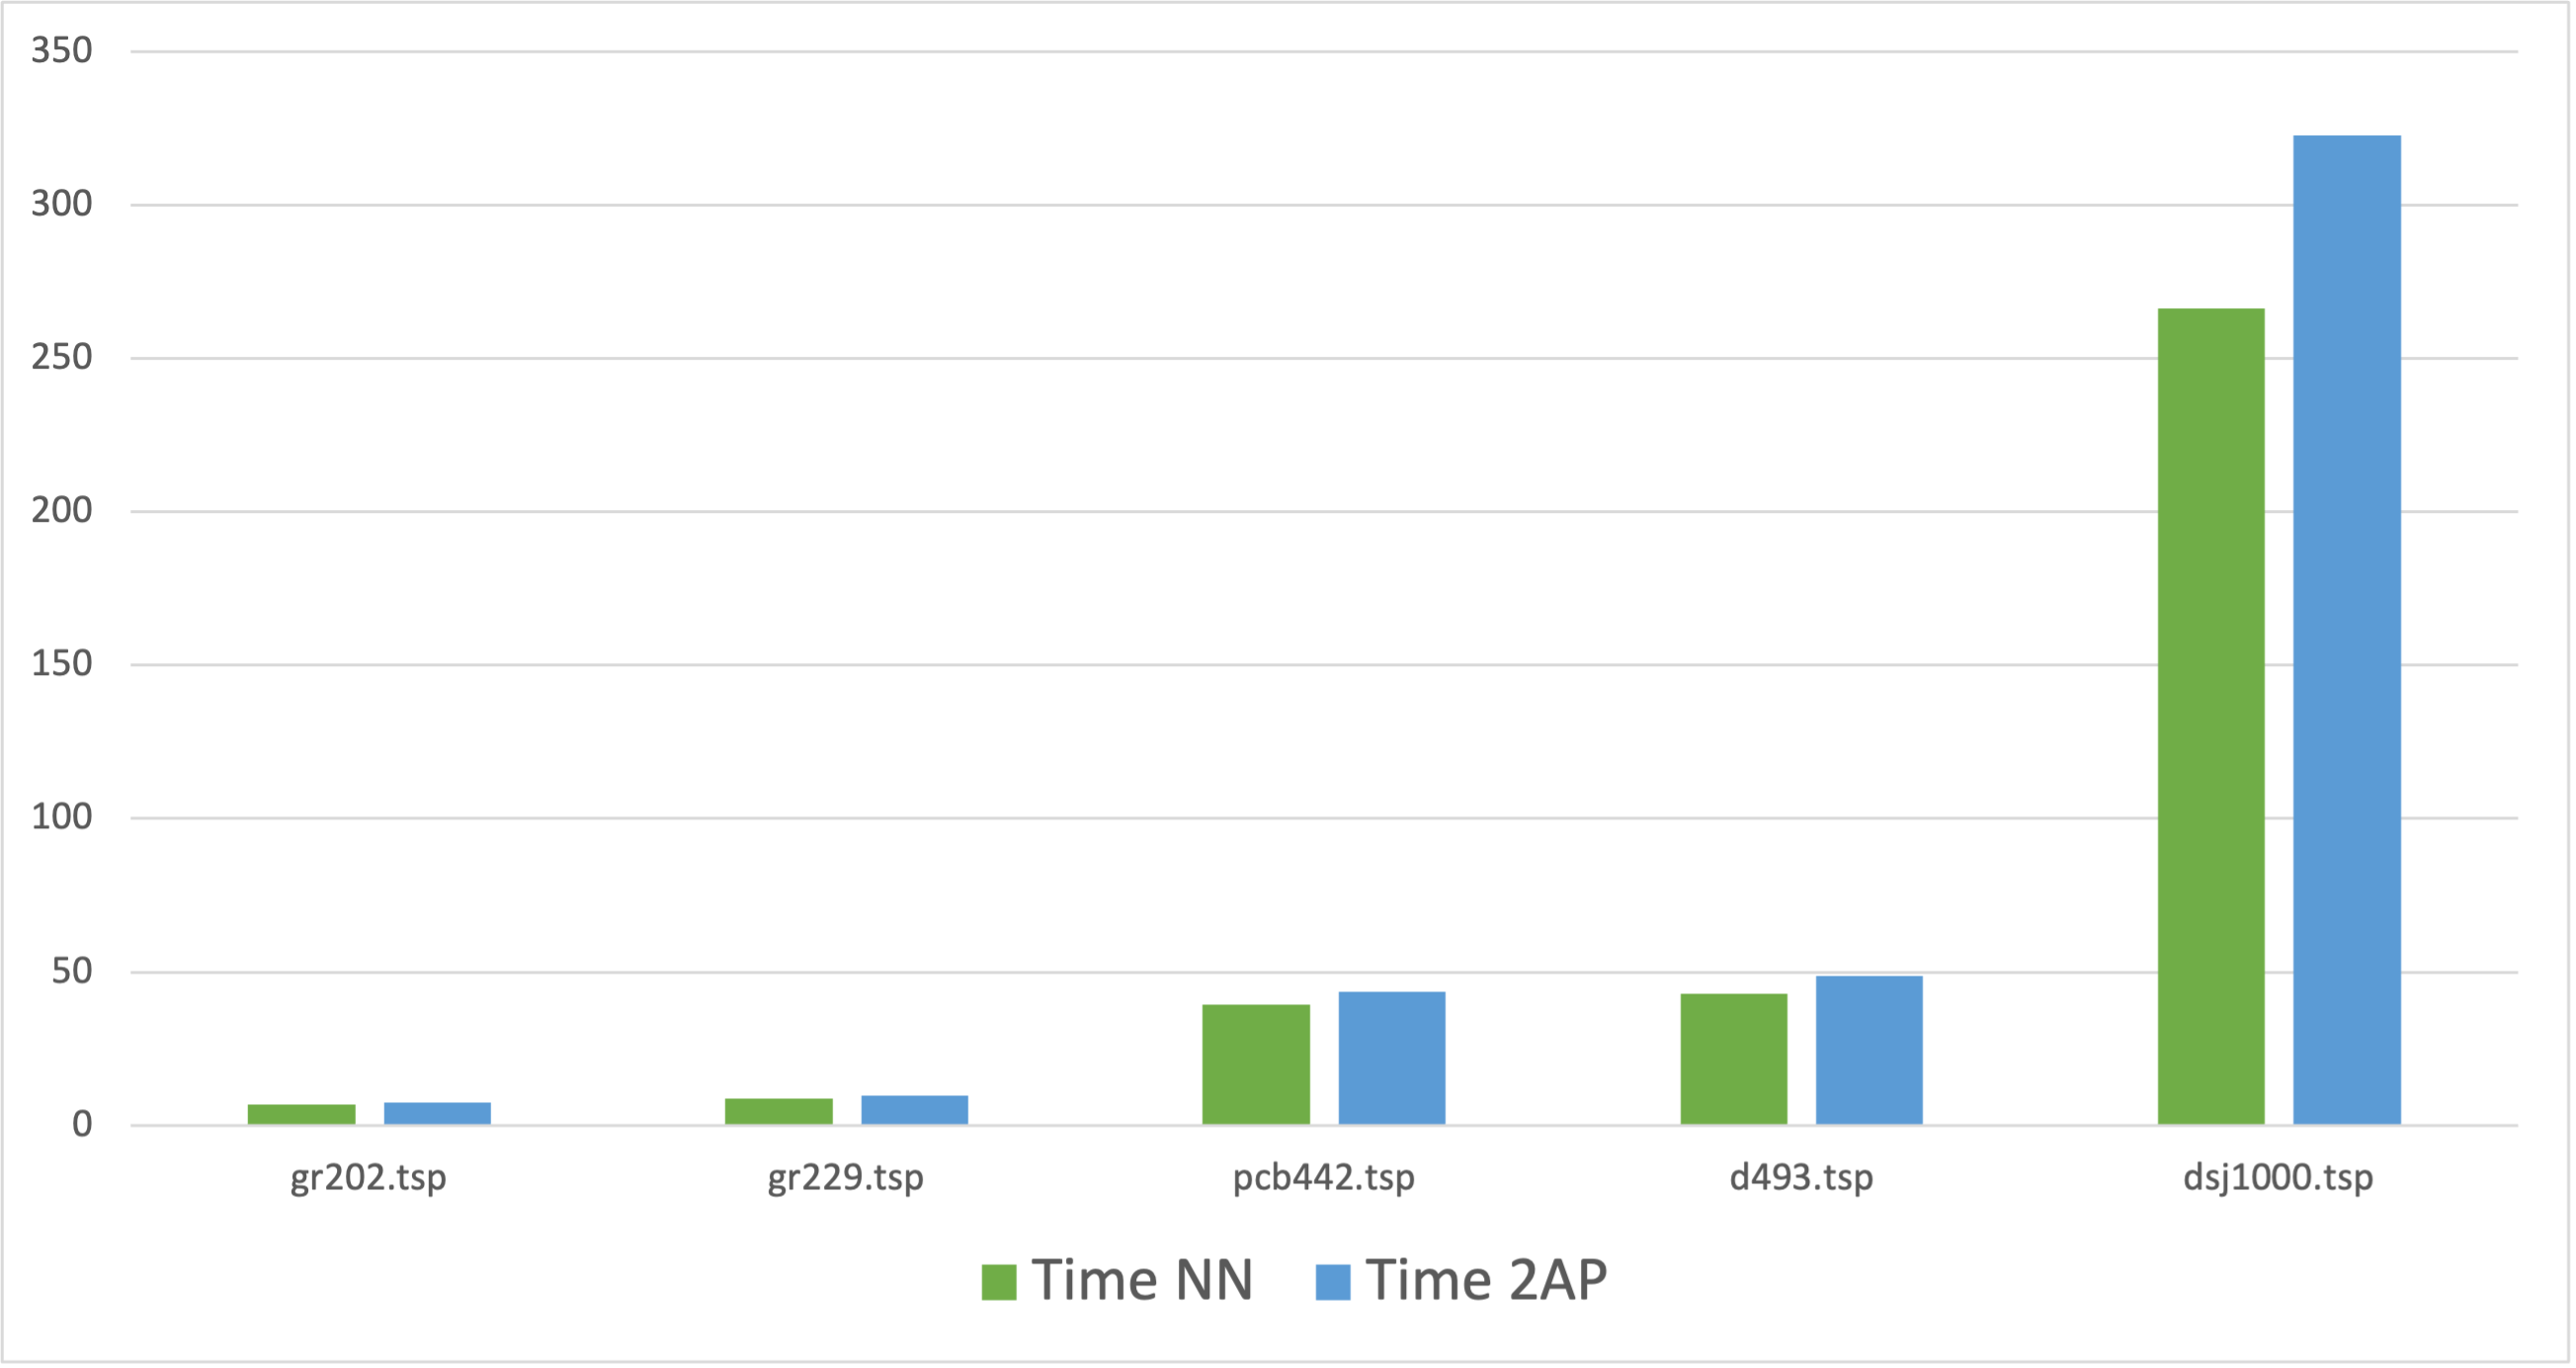
\includegraphics[width=0.9\textwidth]{./img/time_nn_2ap_big.png}
    \caption{Execution time for Nearest Neighbour and 2-Approximation on big dataset.}
    \label{fig:time_nn_2ap_big}
\end{figure}
\noindent
Regarding the execution time of the algorithms, we can see from the graph (fig. \ref{fig:time_nn_2ap_big}), that the execution time of the two algorithms (repeated more than ones), give us a execution time less in the Nearest Neighbor algorithm specially in the bigger graphs.\\
Similarly, also in the smaller graphs (fig. \ref{fig:time_nn_2ap_small}) we noticed that this algorithm take less computational time, confirming itself as the faster of the three.

\begin{figure}[H]
    \centering
    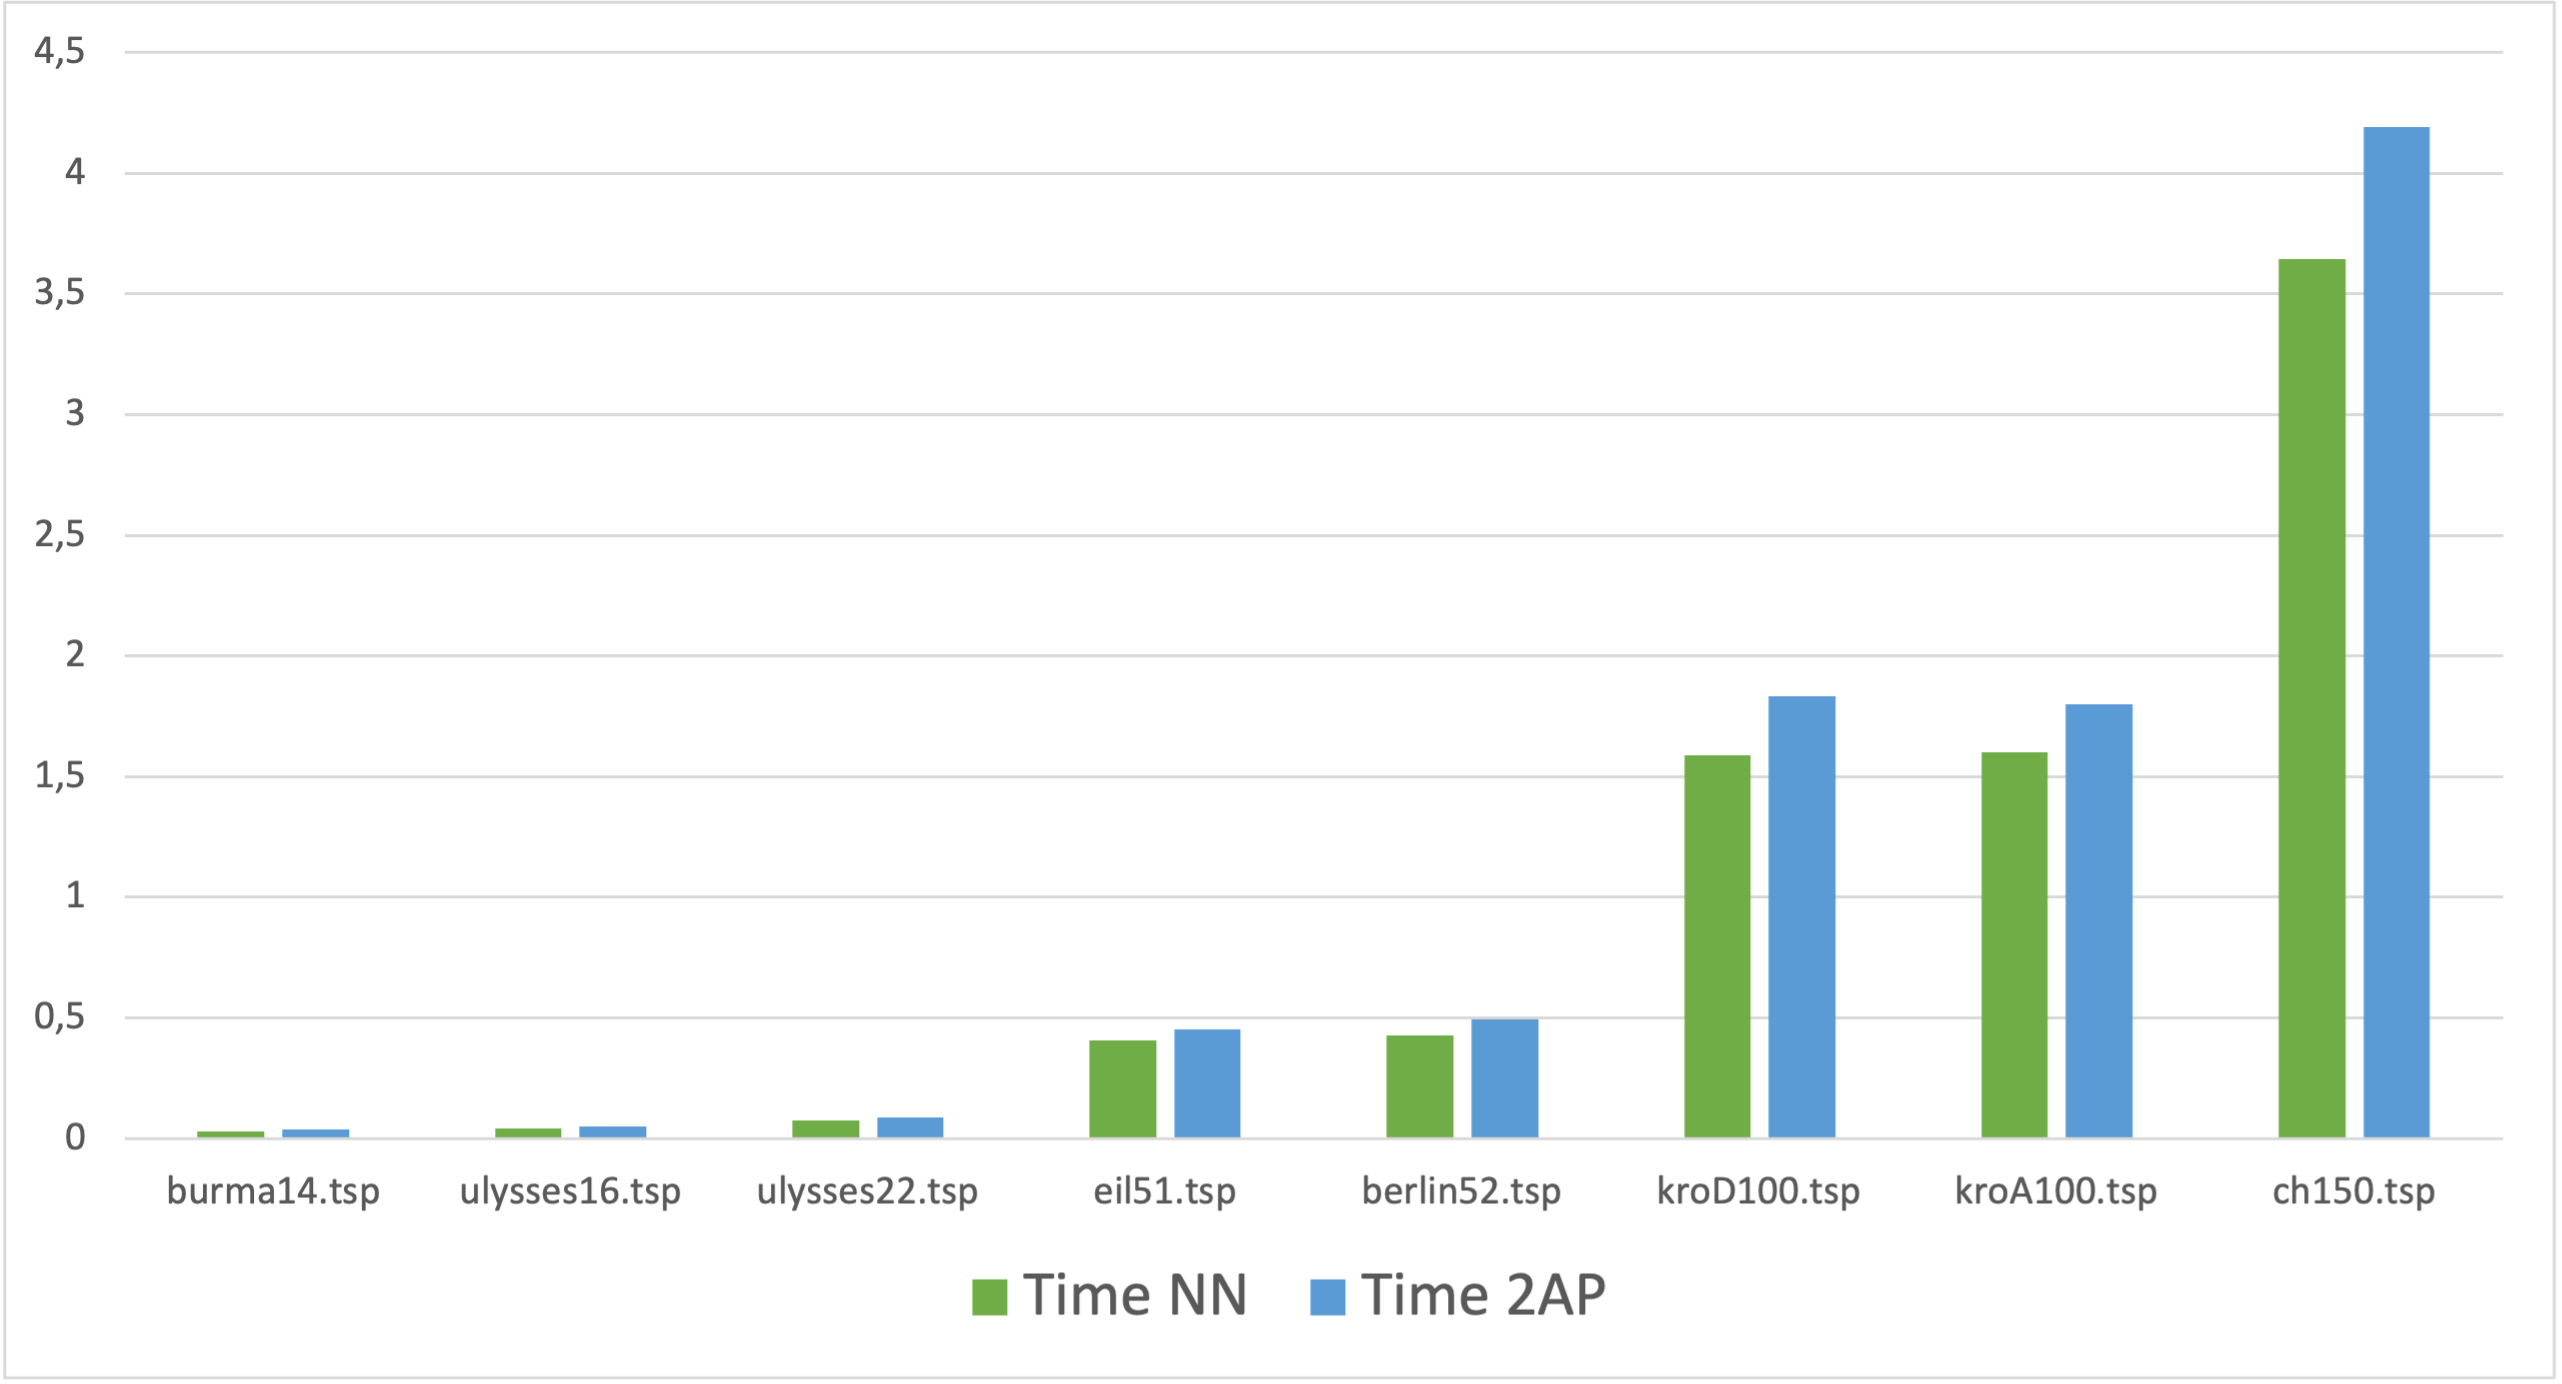
\includegraphics[width=0.9\textwidth]{./img/time_nn_2ap_small.png}
    \caption{Execution time for Nearest Neighbor and 2-Approximation on small dataset.}
    \label{fig:time_nn_2ap_small}
\end{figure}
